\documentclass{article}
\usepackage{graphicx}

\begin{document}
\section{Présentation de l'équipe}
Coc'Otter regroupe des membres de deux anciennes équipes participantes à la coupe : 
\begin{itemize}
\item[--] Cocobot
\item[--] Rob'otter
\end{itemize}
Afin de mutualiser le faible temps restants à de jeunes parents, ce dit temps est mutualisé au sein de la nouvelle équipe : Coc'Otter !

\section{Projet Scientifique et Technique}

Aucune des deux équipe n'ont pas participé à la précédente édition. Ainsi, la PAMI est l'élément qu'aucune équipe n'a jamais conçus.
C'est donc l'objet du projet scientifique et technique.

Un PAMI doit: 
\begin{itemize}
\item[--] être conforme aux règles de la coupe
\item[--] coûter le moins cher possible
\item[--] contenir tout ce qu'un robot standard idéal doit contenir
\item[--] être suffisamment petit pour pouvoir en disposer 10 sur le terrain
\end{itemize}

Nous avons pu concevoir un PAMI avec l'architecture ci dessous:\\
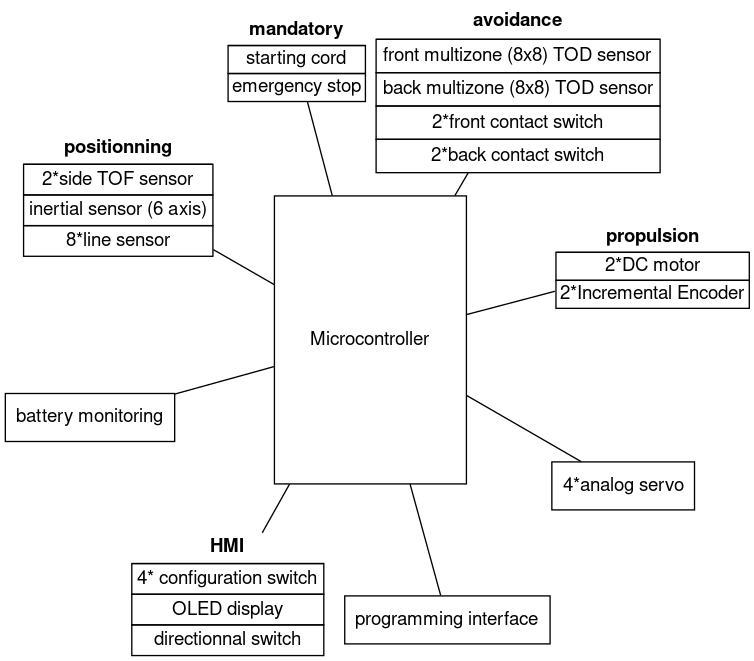
\includegraphics[width = 10cm]{test}

En voici une vue 3D : \\
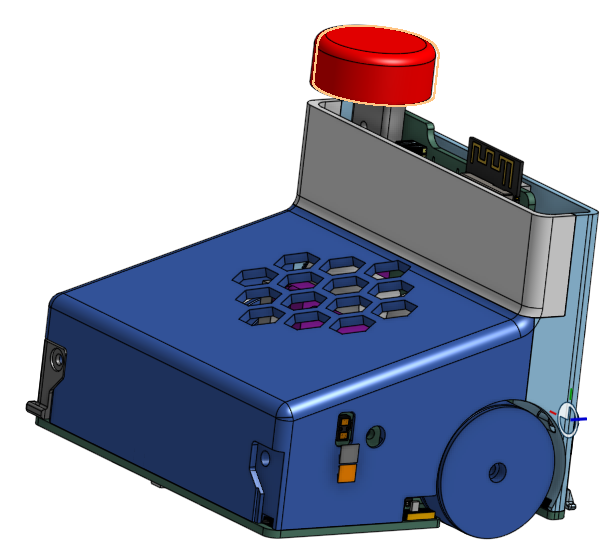
\includegraphics[width = 5cm]{pami_1}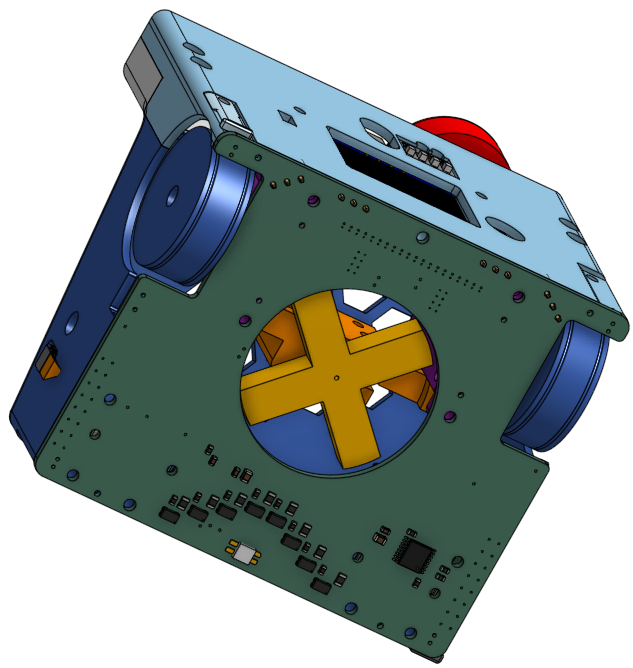
\includegraphics[width = 5cm]{pami_3}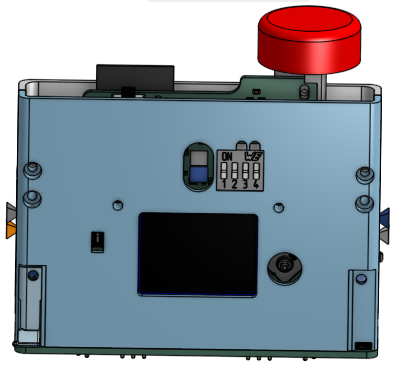
\includegraphics[width = 5cm]{pami_2}
Le PAMI est alimenté par une seule cellule LiFePO4.
Tous les composants électroniques sont montés sur 2 PCB qui constituent une partie de la structure du PAMI.
Les moteurs sont des moteurs de drone montés sur des engrenages de servo moteurs.
Les codeurs incrémentaux sont complètement réalisé par nos soins.
Le PAMI pèse moins de 250g et mesure 85x73x65mm (l*L*h).

Les capteurs TOF doivent permettre de faire du suivi de bordure, et de la détection d'adversaire.
Le gyroscope a été intégré afin de permettre une meilleure localisation du PAMI avec l'utilisation potentielle d'un filtre de KALMAN.

Enfin, ce PAMI est codé en RUST afin de permettre aux membres de l'équipe de monter en compétence sur ce langage.

\section{Plan de Communication}
Il ne faut pas se leurrer, nous ne sommes pas bons pour communiquer.
Ainsi, tous nos designs sont disponible sous Github et OnShape.
Ceci constitue une première étape.

De plus, nous nous rendons régulièrement au sein du local de l'équipe Eirbot. Pour l'instant, nous ne faisons qu'y échanger des idées et nos retours d'expérience. Bien entendu, nous leur avons partagé les liens vers nos dépots Github et design OnShape.
Le PAMI arrive à maturité, l'asserv commence à fonctionner. Ainsi nous allons nous rendre plus régulièrement dans les locaux d'Eirbot pour faire des tests sur terrain. Ce sera l'occasion de mettre en pratique nos connaissance et de démontrer nos belles paroles par des actes.

\end{document}
